



% Seite 6664
According to \citep{Hothorn.2006} an algorithm for recursive partitionig is called unbiased when, under the conditions of the null hypothesis of independence between a response $Y$ an covariates $X_{1},...X_{m}$ the probability of selecting covariate $X_{j}$ is $1/m$ for all $j = 1,...,m$ regardless of the measurement scales or number of missing values. 

\vspace{1cm}

\textbf{Notes on selection bias}

\textit{Warum soll Selection Bias vermieden werden? Was ist eigentlich die Gefahr? 
Zitat von Strobl in \citep{Loh.2014}!: "What we should probably point out more clearly though is that this also means that when
a predictor variable offering few cutpoints is in fact associated with the response—and thus
should be found relevant by any reasonable statistical learning technique—it may still be outperformed by a less informative or even irrelevant competitor, just because the latter offers more cutpoints."}

\textit{Noch deutlicher: "One should think that the results shown here, and in many previous studies that Wei-Yin Loh has summarized in his paper, are so clear that any statistically educated person should never
want to use a biased recursive partitioning algorithm again."}

\textit{Entgegnung von Loh: Selection bias can increase the likelihood of spurious splits on irrelevant variables,
but if the sample size is large and there are not too many such variables, a correspondingly
large tree may subsequently split on the important variables. If the spurious splits survive after
pruning, they simply stratify the data into two or more subsets each having its own subtree, and
overall prediction accuracy may be preserved;}






\vspace{1cm}



%\textbf{Test for selection bias:} $\chi^2$ goodness of fit test\\
%H0: the probabilities of the population are all equal (or are equal to an assumed probability distribution p)

\subsection{Scenario 1: numerical features}
$\textbf{x}_{1}, \textbf{x}_{2} \sim U(0,1)$; 
$\textbf{x}_{3}$ uniformly distributed on the set $(0, 0.1, 0.1,..., 0.9, 1)$;
$\textbf{x}_{4}$ uniformly distributed on the set $(0, 0.01, 0.02,..., 0.99, 1)$;
   
\subsubsection{Independence scenario}
$\textbf{Y} \sim N(0,1)$
\begin{figure}
    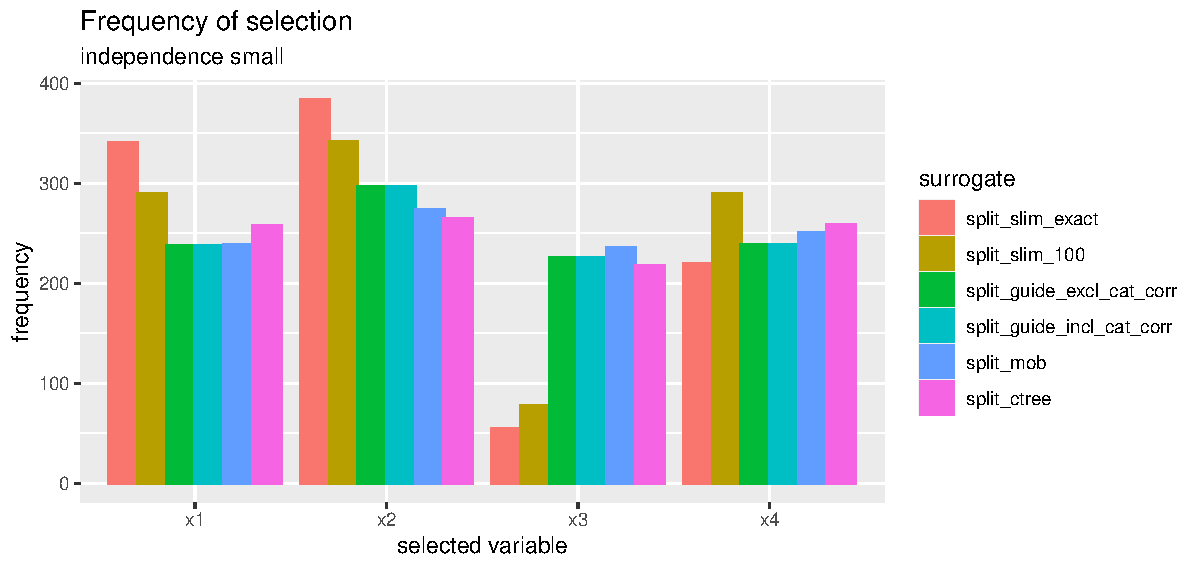
\includegraphics[width=16cm]{Figures/simulations/batchtools/selection_bias_general_10_01/independence_small.pdf}
\end{figure}  
\color{blue} guide nur einmal !
\color{black}
\subsubsection{Interaction scenario}
$Y = \textbf{x}_1\textbf{x}_2 + \textbf{x}_1\textbf{x}_3 + \textbf{x}_1\textbf{x}_4 + \textbf{x}_2\textbf{x}_3 + \textbf{x}_2\textbf{x}_4 + \textbf{x}_3\textbf{x}_4 + \epsilon$ \\
$\epsilon \sim N(0,0.1sd(Y))$
\begin{figure}
    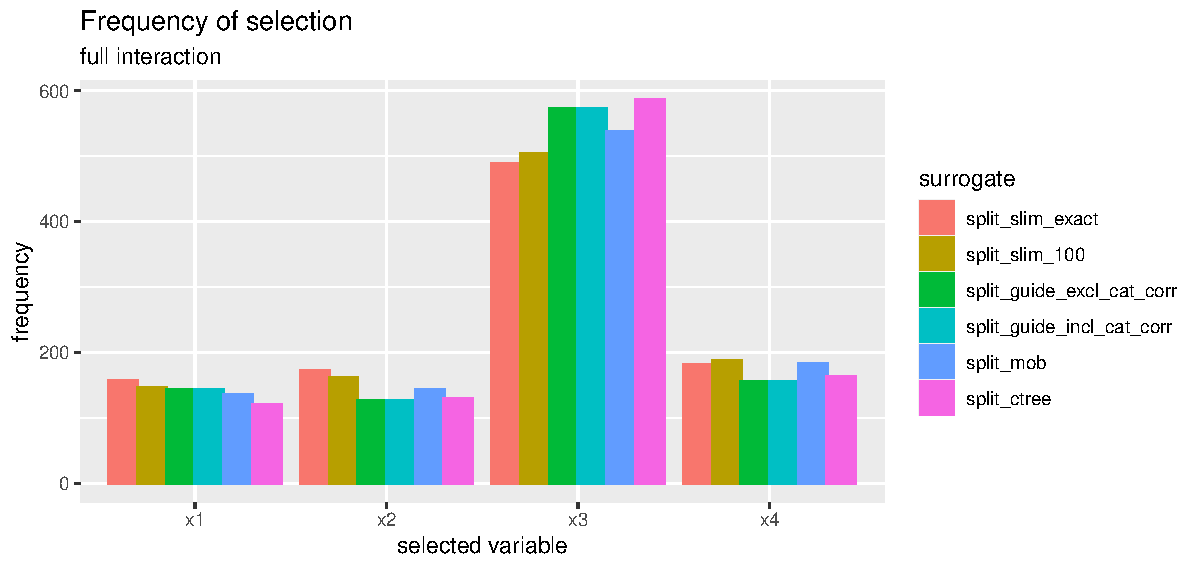
\includegraphics[width=16cm]{Figures/simulations/batchtools/selection_bias_general_10_01/full_interaction.pdf}
\end{figure}  

\subsubsection{SLIM correction approach of selection bias for numerical features}
\begin{figure}
    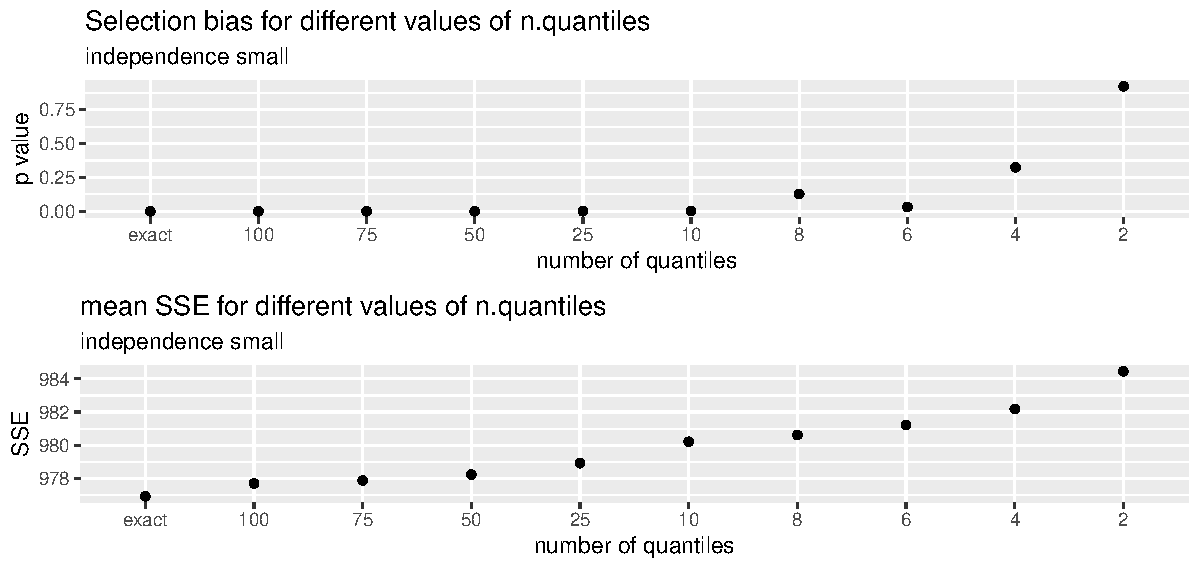
\includegraphics[width=16cm]{Figures/simulations/batchtools/selection_bias_slim/independence_small.pdf}
\end{figure} 


\subsection{Scenario 2: mixed features}
\subsubsection{Independence scenarios}


\subsubsection{Interaction Scenarios}
\begin{itemize}
    \item binary vs. numerical
    \item categorical vs. numerical
\end{itemize}



